% Created by tikzDevice version 0.7.0 on 2014-07-24 03:37:50
% !TEX encoding = UTF-8 Unicode
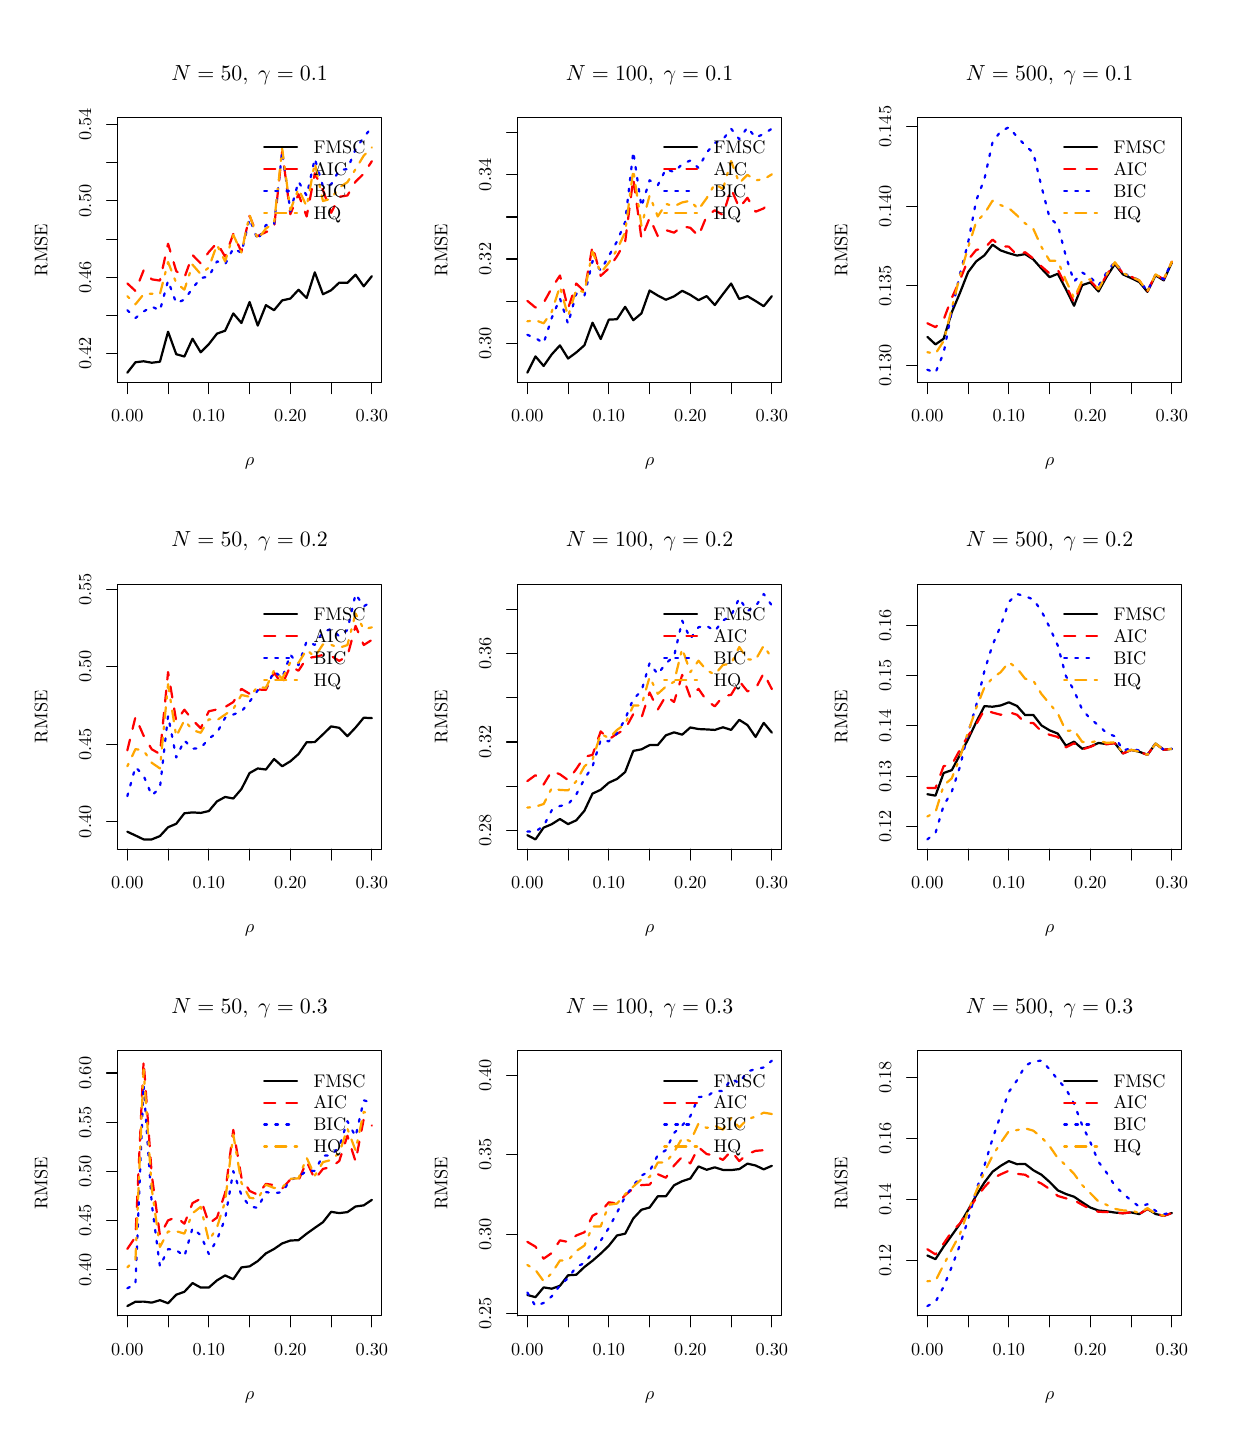
\begin{tikzpicture}[x=1pt,y=1pt]
\definecolor[named]{fillColor}{rgb}{1.00,1.00,1.00}
\path[use as bounding box,fill=fillColor,fill opacity=0.00] (0,0) rectangle (433.62,505.89);
\begin{scope}
\path[clip] ( 32.47,377.65) rectangle (127.91,473.42);
\definecolor[named]{drawColor}{rgb}{0.00,0.00,0.00}

\path[draw=drawColor,line width= 0.8pt,line join=round,line cap=round] ( 36.01,381.20) --
	( 38.95,384.98) --
	( 41.90,385.34) --
	( 44.84,384.81) --
	( 47.79,385.17) --
	( 50.73,396.02) --
	( 53.68,387.89) --
	( 56.63,387.06) --
	( 59.57,393.49) --
	( 62.52,388.58) --
	( 65.46,391.52) --
	( 68.41,395.32) --
	( 71.35,396.38) --
	( 74.30,402.62) --
	( 77.24,399.17) --
	( 80.19,406.75) --
	( 83.14,398.23) --
	( 86.08,405.62) --
	( 89.03,403.79) --
	( 91.97,407.34) --
	( 94.92,407.99) --
	( 97.86,411.17) --
	(100.81,408.20) --
	(103.75,417.47) --
	(106.70,409.56) --
	(109.65,411.00) --
	(112.59,413.76) --
	(115.54,413.68) --
	(118.48,416.61) --
	(121.43,412.43) --
	(124.37,416.09);
\end{scope}
\begin{scope}
\path[clip] (  0.00,  0.00) rectangle (433.62,505.89);
\definecolor[named]{drawColor}{rgb}{0.00,0.00,0.00}

\path[draw=drawColor,line width= 0.4pt,line join=round,line cap=round] ( 36.01,377.65) -- (124.37,377.65);

\path[draw=drawColor,line width= 0.4pt,line join=round,line cap=round] ( 36.01,377.65) -- ( 36.01,373.69);

\path[draw=drawColor,line width= 0.4pt,line join=round,line cap=round] ( 50.73,377.65) -- ( 50.73,373.69);

\path[draw=drawColor,line width= 0.4pt,line join=round,line cap=round] ( 65.46,377.65) -- ( 65.46,373.69);

\path[draw=drawColor,line width= 0.4pt,line join=round,line cap=round] ( 80.19,377.65) -- ( 80.19,373.69);

\path[draw=drawColor,line width= 0.4pt,line join=round,line cap=round] ( 94.92,377.65) -- ( 94.92,373.69);

\path[draw=drawColor,line width= 0.4pt,line join=round,line cap=round] (109.65,377.65) -- (109.65,373.69);

\path[draw=drawColor,line width= 0.4pt,line join=round,line cap=round] (124.37,377.65) -- (124.37,373.69);

\node[text=drawColor,anchor=base,inner sep=0pt, outer sep=0pt, scale=  0.66] at ( 36.01,363.40) {0.00};

\node[text=drawColor,anchor=base,inner sep=0pt, outer sep=0pt, scale=  0.66] at ( 65.46,363.40) {0.10};

\node[text=drawColor,anchor=base,inner sep=0pt, outer sep=0pt, scale=  0.66] at ( 94.92,363.40) {0.20};

\node[text=drawColor,anchor=base,inner sep=0pt, outer sep=0pt, scale=  0.66] at (124.37,363.40) {0.30};

\path[draw=drawColor,line width= 0.4pt,line join=round,line cap=round] ( 32.47,388.12) -- ( 32.47,470.87);

\path[draw=drawColor,line width= 0.4pt,line join=round,line cap=round] ( 32.47,388.12) -- ( 28.51,388.12);

\path[draw=drawColor,line width= 0.4pt,line join=round,line cap=round] ( 32.47,401.91) -- ( 28.51,401.91);

\path[draw=drawColor,line width= 0.4pt,line join=round,line cap=round] ( 32.47,415.70) -- ( 28.51,415.70);

\path[draw=drawColor,line width= 0.4pt,line join=round,line cap=round] ( 32.47,429.49) -- ( 28.51,429.49);

\path[draw=drawColor,line width= 0.4pt,line join=round,line cap=round] ( 32.47,443.29) -- ( 28.51,443.29);

\path[draw=drawColor,line width= 0.4pt,line join=round,line cap=round] ( 32.47,457.08) -- ( 28.51,457.08);

\path[draw=drawColor,line width= 0.4pt,line join=round,line cap=round] ( 32.47,470.87) -- ( 28.51,470.87);

\node[text=drawColor,rotate= 90.00,anchor=base,inner sep=0pt, outer sep=0pt, scale=  0.66] at ( 22.97,388.12) {0.42};

\node[text=drawColor,rotate= 90.00,anchor=base,inner sep=0pt, outer sep=0pt, scale=  0.66] at ( 22.97,415.70) {0.46};

\node[text=drawColor,rotate= 90.00,anchor=base,inner sep=0pt, outer sep=0pt, scale=  0.66] at ( 22.97,443.29) {0.50};

\node[text=drawColor,rotate= 90.00,anchor=base,inner sep=0pt, outer sep=0pt, scale=  0.66] at ( 22.97,470.87) {0.54};

\path[draw=drawColor,line width= 0.4pt,line join=round,line cap=round] ( 32.47,377.65) --
	(127.91,377.65) --
	(127.91,473.42) --
	( 32.47,473.42) --
	( 32.47,377.65);
\end{scope}
\begin{scope}
\path[clip] (  0.00,337.26) rectangle (144.54,505.89);
\definecolor[named]{drawColor}{rgb}{0.00,0.00,0.00}

\node[text=drawColor,anchor=base,inner sep=0pt, outer sep=0pt, scale=  0.79] at ( 80.19,486.92) {\bfseries $N=50, \;\gamma=0.1$};

\node[text=drawColor,anchor=base,inner sep=0pt, outer sep=0pt, scale=  0.66] at ( 80.19,347.56) {$\rho$};

\node[text=drawColor,rotate= 90.00,anchor=base,inner sep=0pt, outer sep=0pt, scale=  0.66] at (  7.13,425.53) {RMSE};
\end{scope}
\begin{scope}
\path[clip] ( 32.47,377.65) rectangle (127.91,473.42);
\definecolor[named]{drawColor}{rgb}{1.00,0.00,0.00}

\path[draw=drawColor,line width= 0.8pt,dash pattern=on 4pt off 4pt ,line join=round,line cap=round] ( 36.01,413.47) --
	( 38.95,410.74) --
	( 41.90,418.20) --
	( 44.84,414.95) --
	( 47.79,414.49) --
	( 50.73,427.81) --
	( 53.68,417.95) --
	( 56.63,415.56) --
	( 59.57,423.72) --
	( 62.52,420.71) --
	( 65.46,424.82) --
	( 68.41,428.12) --
	( 71.35,423.15) --
	( 74.30,431.34) --
	( 77.24,424.91) --
	( 80.19,437.87) --
	( 83.14,430.59) --
	( 86.08,432.01) --
	( 89.03,433.47) --
	( 91.97,461.17) --
	( 94.92,438.48) --
	( 97.86,445.69) --
	(100.81,437.65) --
	(103.75,453.27) --
	(106.70,447.16) --
	(109.65,438.97) --
	(112.59,444.76) --
	(115.54,445.25) --
	(118.48,450.25) --
	(121.43,453.10) --
	(124.37,457.64);
\definecolor[named]{drawColor}{rgb}{0.00,0.00,1.00}

\path[draw=drawColor,line width= 0.8pt,dash pattern=on 1pt off 3pt ,line join=round,line cap=round] ( 36.01,403.79) --
	( 38.95,400.97) --
	( 41.90,403.32) --
	( 44.84,405.11) --
	( 47.79,403.69) --
	( 50.73,414.45) --
	( 53.68,406.37) --
	( 56.63,407.60) --
	( 59.57,411.69) --
	( 62.52,415.40) --
	( 65.46,415.95) --
	( 68.41,421.44) --
	( 71.35,420.40) --
	( 74.30,426.16) --
	( 77.24,424.54) --
	( 80.19,436.86) --
	( 83.14,429.10) --
	( 86.08,434.56) --
	( 89.03,434.61) --
	( 91.97,461.11) --
	( 94.92,439.48) --
	( 97.86,450.29) --
	(100.81,445.19) --
	(103.75,458.58) --
	(106.70,448.52) --
	(109.65,449.25) --
	(112.59,454.42) --
	(115.54,454.78) --
	(118.48,461.93) --
	(121.43,466.30) --
	(124.37,469.87);
\definecolor[named]{drawColor}{rgb}{1.00,0.65,0.00}

\path[draw=drawColor,line width= 0.8pt,dash pattern=on 1pt off 3pt on 4pt off 3pt ,line join=round,line cap=round] ( 36.01,408.85) --
	( 38.95,405.94) --
	( 41.90,409.55) --
	( 44.84,409.75) --
	( 47.79,409.60) --
	( 50.73,421.21) --
	( 53.68,413.62) --
	( 56.63,411.21) --
	( 59.57,420.22) --
	( 62.52,416.86) --
	( 65.46,419.22) --
	( 68.41,427.45) --
	( 71.35,421.42) --
	( 74.30,431.00) --
	( 77.24,424.65) --
	( 80.19,438.20) --
	( 83.14,429.38) --
	( 86.08,433.32) --
	( 89.03,435.27) --
	( 91.97,462.14) --
	( 94.92,439.95) --
	( 97.86,447.64) --
	(100.81,441.28) --
	(103.75,456.96) --
	(106.70,443.24) --
	(109.65,444.12) --
	(112.59,448.16) --
	(115.54,450.05) --
	(118.48,454.76) --
	(121.43,459.63) --
	(124.37,462.58);
\definecolor[named]{drawColor}{rgb}{0.00,0.00,0.00}

\path[draw=drawColor,line width= 0.8pt,line join=round,line cap=round] ( 85.47,462.63) -- ( 97.35,462.63);
\definecolor[named]{drawColor}{rgb}{1.00,0.00,0.00}

\path[draw=drawColor,line width= 0.8pt,dash pattern=on 4pt off 4pt ,line join=round,line cap=round] ( 85.47,454.71) -- ( 97.35,454.71);
\definecolor[named]{drawColor}{rgb}{0.00,0.00,1.00}

\path[draw=drawColor,line width= 0.8pt,dash pattern=on 1pt off 3pt ,line join=round,line cap=round] ( 85.47,446.79) -- ( 97.35,446.79);
\definecolor[named]{drawColor}{rgb}{1.00,0.65,0.00}

\path[draw=drawColor,line width= 0.8pt,dash pattern=on 1pt off 3pt on 4pt off 3pt ,line join=round,line cap=round] ( 85.47,438.87) -- ( 97.35,438.87);
\definecolor[named]{drawColor}{rgb}{0.00,0.00,0.00}

\node[text=drawColor,anchor=base west,inner sep=0pt, outer sep=0pt, scale=  0.66] at (103.29,460.35) {FMSC};

\node[text=drawColor,anchor=base west,inner sep=0pt, outer sep=0pt, scale=  0.66] at (103.29,452.43) {AIC};

\node[text=drawColor,anchor=base west,inner sep=0pt, outer sep=0pt, scale=  0.66] at (103.29,444.51) {BIC};

\node[text=drawColor,anchor=base west,inner sep=0pt, outer sep=0pt, scale=  0.66] at (103.29,436.59) {HQ};
\end{scope}
\begin{scope}
\path[clip] (177.01,377.65) rectangle (272.45,473.42);
\definecolor[named]{drawColor}{rgb}{0.00,0.00,0.00}

\path[draw=drawColor,line width= 0.8pt,line join=round,line cap=round] (180.55,381.20) --
	(183.49,387.11) --
	(186.44,383.64) --
	(189.38,387.84) --
	(192.33,391.09) --
	(195.27,386.34) --
	(198.22,388.51) --
	(201.17,391.11) --
	(204.11,399.28) --
	(207.06,393.38) --
	(210.00,400.39) --
	(212.95,400.53) --
	(215.89,405.01) --
	(218.84,400.17) --
	(221.78,402.64) --
	(224.73,410.91) --
	(227.68,409.10) --
	(230.62,407.57) --
	(233.57,408.79) --
	(236.51,410.80) --
	(239.46,409.33) --
	(242.40,407.41) --
	(245.35,408.89) --
	(248.29,405.66) --
	(251.24,409.62) --
	(254.19,413.43) --
	(257.13,407.84) --
	(260.08,408.87) --
	(263.02,407.12) --
	(265.97,405.23) --
	(268.91,408.87);
\end{scope}
\begin{scope}
\path[clip] (  0.00,  0.00) rectangle (433.62,505.89);
\definecolor[named]{drawColor}{rgb}{0.00,0.00,0.00}

\path[draw=drawColor,line width= 0.4pt,line join=round,line cap=round] (180.55,377.65) -- (268.91,377.65);

\path[draw=drawColor,line width= 0.4pt,line join=round,line cap=round] (180.55,377.65) -- (180.55,373.69);

\path[draw=drawColor,line width= 0.4pt,line join=round,line cap=round] (195.27,377.65) -- (195.27,373.69);

\path[draw=drawColor,line width= 0.4pt,line join=round,line cap=round] (210.00,377.65) -- (210.00,373.69);

\path[draw=drawColor,line width= 0.4pt,line join=round,line cap=round] (224.73,377.65) -- (224.73,373.69);

\path[draw=drawColor,line width= 0.4pt,line join=round,line cap=round] (239.46,377.65) -- (239.46,373.69);

\path[draw=drawColor,line width= 0.4pt,line join=round,line cap=round] (254.19,377.65) -- (254.19,373.69);

\path[draw=drawColor,line width= 0.4pt,line join=round,line cap=round] (268.91,377.65) -- (268.91,373.69);

\node[text=drawColor,anchor=base,inner sep=0pt, outer sep=0pt, scale=  0.66] at (180.55,363.40) {0.00};

\node[text=drawColor,anchor=base,inner sep=0pt, outer sep=0pt, scale=  0.66] at (210.00,363.40) {0.10};

\node[text=drawColor,anchor=base,inner sep=0pt, outer sep=0pt, scale=  0.66] at (239.46,363.40) {0.20};

\node[text=drawColor,anchor=base,inner sep=0pt, outer sep=0pt, scale=  0.66] at (268.91,363.40) {0.30};

\path[draw=drawColor,line width= 0.4pt,line join=round,line cap=round] (177.01,391.86) -- (177.01,467.91);

\path[draw=drawColor,line width= 0.4pt,line join=round,line cap=round] (177.01,391.86) -- (173.05,391.86);

\path[draw=drawColor,line width= 0.4pt,line join=round,line cap=round] (177.01,407.07) -- (173.05,407.07);

\path[draw=drawColor,line width= 0.4pt,line join=round,line cap=round] (177.01,422.28) -- (173.05,422.28);

\path[draw=drawColor,line width= 0.4pt,line join=round,line cap=round] (177.01,437.49) -- (173.05,437.49);

\path[draw=drawColor,line width= 0.4pt,line join=round,line cap=round] (177.01,452.70) -- (173.05,452.70);

\path[draw=drawColor,line width= 0.4pt,line join=round,line cap=round] (177.01,467.91) -- (173.05,467.91);

\node[text=drawColor,rotate= 90.00,anchor=base,inner sep=0pt, outer sep=0pt, scale=  0.66] at (167.51,391.86) {0.30};

\node[text=drawColor,rotate= 90.00,anchor=base,inner sep=0pt, outer sep=0pt, scale=  0.66] at (167.51,422.28) {0.32};

\node[text=drawColor,rotate= 90.00,anchor=base,inner sep=0pt, outer sep=0pt, scale=  0.66] at (167.51,452.70) {0.34};

\path[draw=drawColor,line width= 0.4pt,line join=round,line cap=round] (177.01,377.65) --
	(272.45,377.65) --
	(272.45,473.42) --
	(177.01,473.42) --
	(177.01,377.65);
\end{scope}
\begin{scope}
\path[clip] (144.54,337.26) rectangle (289.08,505.89);
\definecolor[named]{drawColor}{rgb}{0.00,0.00,0.00}

\node[text=drawColor,anchor=base,inner sep=0pt, outer sep=0pt, scale=  0.79] at (224.73,486.92) {\bfseries $N=100, \;\gamma=0.1$};

\node[text=drawColor,anchor=base,inner sep=0pt, outer sep=0pt, scale=  0.66] at (224.73,347.56) {$\rho$};

\node[text=drawColor,rotate= 90.00,anchor=base,inner sep=0pt, outer sep=0pt, scale=  0.66] at (151.67,425.54) {RMSE};
\end{scope}
\begin{scope}
\path[clip] (177.01,377.65) rectangle (272.45,473.42);
\definecolor[named]{drawColor}{rgb}{1.00,0.00,0.00}

\path[draw=drawColor,line width= 0.8pt,dash pattern=on 4pt off 4pt ,line join=round,line cap=round] (180.55,407.18) --
	(183.49,404.75) --
	(186.44,406.47) --
	(189.38,411.79) --
	(192.33,416.34) --
	(195.27,404.38) --
	(198.22,413.42) --
	(201.17,410.60) --
	(204.11,427.01) --
	(207.06,416.20) --
	(210.00,418.93) --
	(212.95,423.33) --
	(215.89,428.44) --
	(218.84,451.38) --
	(221.78,429.68) --
	(224.73,437.17) --
	(227.68,430.61) --
	(230.62,432.74) --
	(233.57,431.81) --
	(236.51,434.10) --
	(239.46,433.57) --
	(242.40,430.58) --
	(245.35,437.81) --
	(248.29,439.90) --
	(251.24,438.19) --
	(254.19,447.67) --
	(257.13,440.79) --
	(260.08,444.41) --
	(263.02,439.38) --
	(265.97,440.58) --
	(268.91,443.79);
\definecolor[named]{drawColor}{rgb}{0.00,0.00,1.00}

\path[draw=drawColor,line width= 0.8pt,dash pattern=on 1pt off 3pt ,line join=round,line cap=round] (180.55,394.90) --
	(183.49,393.74) --
	(186.44,391.87) --
	(189.38,401.03) --
	(192.33,408.03) --
	(195.27,398.87) --
	(198.22,409.77) --
	(201.17,408.97) --
	(204.11,421.56) --
	(207.06,418.19) --
	(210.00,423.38) --
	(212.95,428.65) --
	(215.89,435.65) --
	(218.84,461.07) --
	(221.78,441.21) --
	(224.73,450.74) --
	(227.68,448.92) --
	(230.62,454.81) --
	(233.57,453.68) --
	(236.51,456.61) --
	(239.46,457.87) --
	(242.40,455.19) --
	(245.35,460.72) --
	(248.29,464.23) --
	(251.24,465.49) --
	(254.19,469.37) --
	(257.13,465.59) --
	(260.08,469.87) --
	(263.02,466.16) --
	(265.97,467.48) --
	(268.91,469.39);
\definecolor[named]{drawColor}{rgb}{1.00,0.65,0.00}

\path[draw=drawColor,line width= 0.8pt,dash pattern=on 1pt off 3pt on 4pt off 3pt ,line join=round,line cap=round] (180.55,399.78) --
	(183.49,400.16) --
	(186.44,399.06) --
	(189.38,403.25) --
	(192.33,412.39) --
	(195.27,401.58) --
	(198.22,411.26) --
	(201.17,410.27) --
	(204.11,424.98) --
	(207.06,417.30) --
	(210.00,420.93) --
	(212.95,425.64) --
	(215.89,431.96) --
	(218.84,454.55) --
	(221.78,434.33) --
	(224.73,445.22) --
	(227.68,437.67) --
	(230.62,442.22) --
	(233.57,441.35) --
	(236.51,442.74) --
	(239.46,443.36) --
	(242.40,440.17) --
	(245.35,444.27) --
	(248.29,449.42) --
	(251.24,447.59) --
	(254.19,457.66) --
	(257.13,449.73) --
	(260.08,452.70) --
	(263.02,450.73) --
	(265.97,451.08) --
	(268.91,452.89);
\definecolor[named]{drawColor}{rgb}{0.00,0.00,0.00}

\path[draw=drawColor,line width= 0.8pt,line join=round,line cap=round] (230.01,462.63) -- (241.89,462.63);
\definecolor[named]{drawColor}{rgb}{1.00,0.00,0.00}

\path[draw=drawColor,line width= 0.8pt,dash pattern=on 4pt off 4pt ,line join=round,line cap=round] (230.01,454.71) -- (241.89,454.71);
\definecolor[named]{drawColor}{rgb}{0.00,0.00,1.00}

\path[draw=drawColor,line width= 0.8pt,dash pattern=on 1pt off 3pt ,line join=round,line cap=round] (230.01,446.79) -- (241.89,446.79);
\definecolor[named]{drawColor}{rgb}{1.00,0.65,0.00}

\path[draw=drawColor,line width= 0.8pt,dash pattern=on 1pt off 3pt on 4pt off 3pt ,line join=round,line cap=round] (230.01,438.87) -- (241.89,438.87);
\definecolor[named]{drawColor}{rgb}{0.00,0.00,0.00}

\node[text=drawColor,anchor=base west,inner sep=0pt, outer sep=0pt, scale=  0.66] at (247.83,460.35) {FMSC};

\node[text=drawColor,anchor=base west,inner sep=0pt, outer sep=0pt, scale=  0.66] at (247.83,452.43) {AIC};

\node[text=drawColor,anchor=base west,inner sep=0pt, outer sep=0pt, scale=  0.66] at (247.83,444.51) {BIC};

\node[text=drawColor,anchor=base west,inner sep=0pt, outer sep=0pt, scale=  0.66] at (247.83,436.59) {HQ};
\end{scope}
\begin{scope}
\path[clip] (321.55,377.65) rectangle (416.99,473.42);
\definecolor[named]{drawColor}{rgb}{0.00,0.00,0.00}

\path[draw=drawColor,line width= 0.8pt,line join=round,line cap=round] (325.09,394.18) --
	(328.03,391.44) --
	(330.98,393.48) --
	(333.92,403.03) --
	(336.87,410.03) --
	(339.81,417.53) --
	(342.76,421.46) --
	(345.71,423.61) --
	(348.65,427.47) --
	(351.60,425.38) --
	(354.54,424.38) --
	(357.49,423.54) --
	(360.43,424.06) --
	(363.38,422.15) --
	(366.32,418.84) --
	(369.27,415.73) --
	(372.22,416.96) --
	(375.16,411.38) --
	(378.11,405.40) --
	(381.05,412.85) --
	(384.00,413.83) --
	(386.94,410.56) --
	(389.89,415.89) --
	(392.83,420.44) --
	(395.78,416.72) --
	(398.73,415.39) --
	(401.67,413.98) --
	(404.62,410.42) --
	(407.56,416.40) --
	(410.51,414.57) --
	(413.45,421.03);
\end{scope}
\begin{scope}
\path[clip] (  0.00,  0.00) rectangle (433.62,505.89);
\definecolor[named]{drawColor}{rgb}{0.00,0.00,0.00}

\path[draw=drawColor,line width= 0.4pt,line join=round,line cap=round] (325.09,377.65) -- (413.45,377.65);

\path[draw=drawColor,line width= 0.4pt,line join=round,line cap=round] (325.09,377.65) -- (325.09,373.69);

\path[draw=drawColor,line width= 0.4pt,line join=round,line cap=round] (339.81,377.65) -- (339.81,373.69);

\path[draw=drawColor,line width= 0.4pt,line join=round,line cap=round] (354.54,377.65) -- (354.54,373.69);

\path[draw=drawColor,line width= 0.4pt,line join=round,line cap=round] (369.27,377.65) -- (369.27,373.69);

\path[draw=drawColor,line width= 0.4pt,line join=round,line cap=round] (384.00,377.65) -- (384.00,373.69);

\path[draw=drawColor,line width= 0.4pt,line join=round,line cap=round] (398.73,377.65) -- (398.73,373.69);

\path[draw=drawColor,line width= 0.4pt,line join=round,line cap=round] (413.45,377.65) -- (413.45,373.69);

\node[text=drawColor,anchor=base,inner sep=0pt, outer sep=0pt, scale=  0.66] at (325.09,363.40) {0.00};

\node[text=drawColor,anchor=base,inner sep=0pt, outer sep=0pt, scale=  0.66] at (354.54,363.40) {0.10};

\node[text=drawColor,anchor=base,inner sep=0pt, outer sep=0pt, scale=  0.66] at (384.00,363.40) {0.20};

\node[text=drawColor,anchor=base,inner sep=0pt, outer sep=0pt, scale=  0.66] at (413.45,363.40) {0.30};

\path[draw=drawColor,line width= 0.4pt,line join=round,line cap=round] (321.55,383.83) -- (321.55,470.13);

\path[draw=drawColor,line width= 0.4pt,line join=round,line cap=round] (321.55,383.83) -- (317.59,383.83);

\path[draw=drawColor,line width= 0.4pt,line join=round,line cap=round] (321.55,412.60) -- (317.59,412.60);

\path[draw=drawColor,line width= 0.4pt,line join=round,line cap=round] (321.55,441.37) -- (317.59,441.37);

\path[draw=drawColor,line width= 0.4pt,line join=round,line cap=round] (321.55,470.13) -- (317.59,470.13);

\node[text=drawColor,rotate= 90.00,anchor=base,inner sep=0pt, outer sep=0pt, scale=  0.66] at (312.05,383.83) {0.130};

\node[text=drawColor,rotate= 90.00,anchor=base,inner sep=0pt, outer sep=0pt, scale=  0.66] at (312.05,412.60) {0.135};

\node[text=drawColor,rotate= 90.00,anchor=base,inner sep=0pt, outer sep=0pt, scale=  0.66] at (312.05,441.37) {0.140};

\node[text=drawColor,rotate= 90.00,anchor=base,inner sep=0pt, outer sep=0pt, scale=  0.66] at (312.05,470.13) {0.145};

\path[draw=drawColor,line width= 0.4pt,line join=round,line cap=round] (321.55,377.65) --
	(416.99,377.65) --
	(416.99,473.42) --
	(321.55,473.42) --
	(321.55,377.65);
\end{scope}
\begin{scope}
\path[clip] (289.08,337.26) rectangle (433.62,505.89);
\definecolor[named]{drawColor}{rgb}{0.00,0.00,0.00}

\node[text=drawColor,anchor=base,inner sep=0pt, outer sep=0pt, scale=  0.79] at (369.27,486.92) {\bfseries $N=500, \;\gamma=0.1$};

\node[text=drawColor,anchor=base,inner sep=0pt, outer sep=0pt, scale=  0.66] at (369.27,347.56) {$\rho$};

\node[text=drawColor,rotate= 90.00,anchor=base,inner sep=0pt, outer sep=0pt, scale=  0.66] at (296.21,425.54) {RMSE};
\end{scope}
\begin{scope}
\path[clip] (321.55,377.65) rectangle (416.99,473.42);
\definecolor[named]{drawColor}{rgb}{1.00,0.00,0.00}

\path[draw=drawColor,line width= 0.8pt,dash pattern=on 4pt off 4pt ,line join=round,line cap=round] (325.09,399.08) --
	(328.03,397.66) --
	(330.98,400.41) --
	(333.92,408.23) --
	(336.87,414.70) --
	(339.81,421.97) --
	(342.76,425.59) --
	(345.71,426.13) --
	(348.65,429.30) --
	(351.60,426.97) --
	(354.54,426.75) --
	(357.49,423.76) --
	(360.43,424.75) --
	(363.38,422.46) --
	(366.32,419.63) --
	(369.27,417.07) --
	(372.22,418.39) --
	(375.16,412.72) --
	(378.11,406.61) --
	(381.05,414.30) --
	(384.00,414.42) --
	(386.94,411.20) --
	(389.89,416.60) --
	(392.83,421.02) --
	(395.78,417.09) --
	(398.73,415.90) --
	(401.67,414.53) --
	(404.62,410.63) --
	(407.56,416.74) --
	(410.51,414.95) --
	(413.45,421.35);
\definecolor[named]{drawColor}{rgb}{0.00,0.00,1.00}

\path[draw=drawColor,line width= 0.8pt,dash pattern=on 1pt off 3pt ,line join=round,line cap=round] (325.09,382.29) --
	(328.03,381.20) --
	(330.98,388.37) --
	(333.92,403.40) --
	(336.87,416.83) --
	(339.81,428.18) --
	(342.76,443.50) --
	(345.71,451.18) --
	(348.65,464.46) --
	(351.60,468.48) --
	(354.54,469.87) --
	(357.49,466.46) --
	(360.43,463.37) --
	(363.38,460.67) --
	(366.32,448.55) --
	(369.27,437.19) --
	(372.22,434.58) --
	(375.16,423.25) --
	(378.11,414.13) --
	(381.05,417.40) --
	(384.00,415.74) --
	(386.94,412.63) --
	(389.89,417.43) --
	(392.83,421.31) --
	(395.78,417.27) --
	(398.73,415.87) --
	(401.67,414.65) --
	(404.62,410.64) --
	(407.56,416.74) --
	(410.51,414.95) --
	(413.45,421.35);
\definecolor[named]{drawColor}{rgb}{1.00,0.65,0.00}

\path[draw=drawColor,line width= 0.8pt,dash pattern=on 1pt off 3pt on 4pt off 3pt ,line join=round,line cap=round] (325.09,388.62) --
	(328.03,388.07) --
	(330.98,392.65) --
	(333.92,404.52) --
	(336.87,416.20) --
	(339.81,426.48) --
	(342.76,435.71) --
	(345.71,438.65) --
	(348.65,443.37) --
	(351.60,441.74) --
	(354.54,440.71) --
	(357.49,438.04) --
	(360.43,435.17) --
	(363.38,433.20) --
	(366.32,426.66) --
	(369.27,421.69) --
	(372.22,421.60) --
	(375.16,414.56) --
	(378.11,408.16) --
	(381.05,414.49) --
	(384.00,414.96) --
	(386.94,411.41) --
	(389.89,416.71) --
	(392.83,421.13) --
	(395.78,417.18) --
	(398.73,415.90) --
	(401.67,414.55) --
	(404.62,410.63) --
	(407.56,416.74) --
	(410.51,414.95) --
	(413.45,421.35);
\definecolor[named]{drawColor}{rgb}{0.00,0.00,0.00}

\path[draw=drawColor,line width= 0.8pt,line join=round,line cap=round] (374.55,462.63) -- (386.43,462.63);
\definecolor[named]{drawColor}{rgb}{1.00,0.00,0.00}

\path[draw=drawColor,line width= 0.8pt,dash pattern=on 4pt off 4pt ,line join=round,line cap=round] (374.55,454.71) -- (386.43,454.71);
\definecolor[named]{drawColor}{rgb}{0.00,0.00,1.00}

\path[draw=drawColor,line width= 0.8pt,dash pattern=on 1pt off 3pt ,line join=round,line cap=round] (374.55,446.79) -- (386.43,446.79);
\definecolor[named]{drawColor}{rgb}{1.00,0.65,0.00}

\path[draw=drawColor,line width= 0.8pt,dash pattern=on 1pt off 3pt on 4pt off 3pt ,line join=round,line cap=round] (374.55,438.87) -- (386.43,438.87);
\definecolor[named]{drawColor}{rgb}{0.00,0.00,0.00}

\node[text=drawColor,anchor=base west,inner sep=0pt, outer sep=0pt, scale=  0.66] at (392.37,460.35) {FMSC};

\node[text=drawColor,anchor=base west,inner sep=0pt, outer sep=0pt, scale=  0.66] at (392.37,452.43) {AIC};

\node[text=drawColor,anchor=base west,inner sep=0pt, outer sep=0pt, scale=  0.66] at (392.37,444.51) {BIC};

\node[text=drawColor,anchor=base west,inner sep=0pt, outer sep=0pt, scale=  0.66] at (392.37,436.59) {HQ};
\end{scope}
\begin{scope}
\path[clip] ( 32.47,209.02) rectangle (127.91,304.79);
\definecolor[named]{drawColor}{rgb}{0.00,0.00,0.00}

\path[draw=drawColor,line width= 0.8pt,line join=round,line cap=round] ( 36.01,215.35) --
	( 38.95,213.98) --
	( 41.90,212.57) --
	( 44.84,212.57) --
	( 47.79,213.77) --
	( 50.73,216.96) --
	( 53.68,218.21) --
	( 56.63,222.01) --
	( 59.57,222.33) --
	( 62.52,222.14) --
	( 65.46,222.81) --
	( 68.41,226.31) --
	( 71.35,227.92) --
	( 74.30,227.34) --
	( 77.24,230.76) --
	( 80.19,236.55) --
	( 83.14,238.20) --
	( 86.08,237.82) --
	( 89.03,241.62) --
	( 91.97,238.99) --
	( 94.92,240.79) --
	( 97.86,243.39) --
	(100.81,247.68) --
	(103.75,247.73) --
	(106.70,250.53) --
	(109.65,253.40) --
	(112.59,252.89) --
	(115.54,249.86) --
	(118.48,252.98) --
	(121.43,256.53) --
	(124.37,256.41);
\end{scope}
\begin{scope}
\path[clip] (  0.00,  0.00) rectangle (433.62,505.89);
\definecolor[named]{drawColor}{rgb}{0.00,0.00,0.00}

\path[draw=drawColor,line width= 0.4pt,line join=round,line cap=round] ( 36.01,209.02) -- (124.37,209.02);

\path[draw=drawColor,line width= 0.4pt,line join=round,line cap=round] ( 36.01,209.02) -- ( 36.01,205.06);

\path[draw=drawColor,line width= 0.4pt,line join=round,line cap=round] ( 50.73,209.02) -- ( 50.73,205.06);

\path[draw=drawColor,line width= 0.4pt,line join=round,line cap=round] ( 65.46,209.02) -- ( 65.46,205.06);

\path[draw=drawColor,line width= 0.4pt,line join=round,line cap=round] ( 80.19,209.02) -- ( 80.19,205.06);

\path[draw=drawColor,line width= 0.4pt,line join=round,line cap=round] ( 94.92,209.02) -- ( 94.92,205.06);

\path[draw=drawColor,line width= 0.4pt,line join=round,line cap=round] (109.65,209.02) -- (109.65,205.06);

\path[draw=drawColor,line width= 0.4pt,line join=round,line cap=round] (124.37,209.02) -- (124.37,205.06);

\node[text=drawColor,anchor=base,inner sep=0pt, outer sep=0pt, scale=  0.66] at ( 36.01,194.77) {0.00};

\node[text=drawColor,anchor=base,inner sep=0pt, outer sep=0pt, scale=  0.66] at ( 65.46,194.77) {0.10};

\node[text=drawColor,anchor=base,inner sep=0pt, outer sep=0pt, scale=  0.66] at ( 94.92,194.77) {0.20};

\node[text=drawColor,anchor=base,inner sep=0pt, outer sep=0pt, scale=  0.66] at (124.37,194.77) {0.30};

\path[draw=drawColor,line width= 0.4pt,line join=round,line cap=round] ( 32.47,218.91) -- ( 32.47,302.99);

\path[draw=drawColor,line width= 0.4pt,line join=round,line cap=round] ( 32.47,218.91) -- ( 28.51,218.91);

\path[draw=drawColor,line width= 0.4pt,line join=round,line cap=round] ( 32.47,246.94) -- ( 28.51,246.94);

\path[draw=drawColor,line width= 0.4pt,line join=round,line cap=round] ( 32.47,274.97) -- ( 28.51,274.97);

\path[draw=drawColor,line width= 0.4pt,line join=round,line cap=round] ( 32.47,302.99) -- ( 28.51,302.99);

\node[text=drawColor,rotate= 90.00,anchor=base,inner sep=0pt, outer sep=0pt, scale=  0.66] at ( 22.97,218.91) {0.40};

\node[text=drawColor,rotate= 90.00,anchor=base,inner sep=0pt, outer sep=0pt, scale=  0.66] at ( 22.97,246.94) {0.45};

\node[text=drawColor,rotate= 90.00,anchor=base,inner sep=0pt, outer sep=0pt, scale=  0.66] at ( 22.97,274.97) {0.50};

\node[text=drawColor,rotate= 90.00,anchor=base,inner sep=0pt, outer sep=0pt, scale=  0.66] at ( 22.97,302.99) {0.55};

\path[draw=drawColor,line width= 0.4pt,line join=round,line cap=round] ( 32.47,209.02) --
	(127.91,209.02) --
	(127.91,304.79) --
	( 32.47,304.79) --
	( 32.47,209.02);
\end{scope}
\begin{scope}
\path[clip] (  0.00,168.63) rectangle (144.54,337.26);
\definecolor[named]{drawColor}{rgb}{0.00,0.00,0.00}

\node[text=drawColor,anchor=base,inner sep=0pt, outer sep=0pt, scale=  0.79] at ( 80.19,318.29) {\bfseries $N=50, \;\gamma=0.2$};

\node[text=drawColor,anchor=base,inner sep=0pt, outer sep=0pt, scale=  0.66] at ( 80.19,178.93) {$\rho$};

\node[text=drawColor,rotate= 90.00,anchor=base,inner sep=0pt, outer sep=0pt, scale=  0.66] at (  7.13,256.90) {RMSE};
\end{scope}
\begin{scope}
\path[clip] ( 32.47,209.02) rectangle (127.91,304.79);
\definecolor[named]{drawColor}{rgb}{1.00,0.00,0.00}

\path[draw=drawColor,line width= 0.8pt,dash pattern=on 4pt off 4pt ,line join=round,line cap=round] ( 36.01,244.74) --
	( 38.95,256.81) --
	( 41.90,250.02) --
	( 44.84,245.13) --
	( 47.79,243.41) --
	( 50.73,273.03) --
	( 53.68,255.32) --
	( 56.63,259.44) --
	( 59.57,255.68) --
	( 62.52,252.73) --
	( 65.46,258.87) --
	( 68.41,259.53) --
	( 71.35,260.40) --
	( 74.30,262.20) --
	( 77.24,266.96) --
	( 80.19,265.18) --
	( 83.14,266.74) --
	( 86.08,266.59) --
	( 89.03,272.80) --
	( 91.97,268.56) --
	( 94.92,275.16) --
	( 97.86,273.52) --
	(100.81,278.03) --
	(103.75,278.51) --
	(106.70,279.21) --
	(109.65,278.86) --
	(112.59,277.08) --
	(115.54,278.82) --
	(118.48,289.71) --
	(121.43,282.81) --
	(124.37,284.65);
\definecolor[named]{drawColor}{rgb}{0.00,0.00,1.00}

\path[draw=drawColor,line width= 0.8pt,dash pattern=on 1pt off 3pt ,line join=round,line cap=round] ( 36.01,228.20) --
	( 38.95,238.75) --
	( 41.90,235.58) --
	( 44.84,228.48) --
	( 47.79,231.13) --
	( 50.73,257.24) --
	( 53.68,242.17) --
	( 56.63,248.35) --
	( 59.57,245.33) --
	( 62.52,245.58) --
	( 65.46,248.97) --
	( 68.41,251.11) --
	( 71.35,256.50) --
	( 74.30,257.69) --
	( 77.24,258.78) --
	( 80.19,262.31) --
	( 83.14,266.44) --
	( 86.08,267.09) --
	( 89.03,273.35) --
	( 91.97,270.90) --
	( 94.92,279.35) --
	( 97.86,275.51) --
	(100.81,284.15) --
	(103.75,282.85) --
	(106.70,287.58) --
	(109.65,288.59) --
	(112.59,285.96) --
	(115.54,288.23) --
	(118.48,301.24) --
	(121.43,296.79) --
	(124.37,298.51);
\definecolor[named]{drawColor}{rgb}{1.00,0.65,0.00}

\path[draw=drawColor,line width= 0.8pt,dash pattern=on 1pt off 3pt on 4pt off 3pt ,line join=round,line cap=round] ( 36.01,238.99) --
	( 38.95,245.20) --
	( 41.90,244.69) --
	( 44.84,240.25) --
	( 47.79,238.22) --
	( 50.73,268.67) --
	( 53.68,249.76) --
	( 56.63,255.63) --
	( 59.57,252.11) --
	( 62.52,251.09) --
	( 65.46,255.97) --
	( 68.41,255.64) --
	( 71.35,257.67) --
	( 74.30,259.68) --
	( 77.24,264.77) --
	( 80.19,264.11) --
	( 83.14,267.81) --
	( 86.08,267.27) --
	( 89.03,273.68) --
	( 91.97,270.59) --
	( 94.92,276.57) --
	( 97.86,276.40) --
	(100.81,281.07) --
	(103.75,278.55) --
	(106.70,283.04) --
	(109.65,282.86) --
	(112.59,281.79) --
	(115.54,282.80) --
	(118.48,294.18) --
	(121.43,288.53) --
	(124.37,289.20);
\definecolor[named]{drawColor}{rgb}{0.00,0.00,0.00}

\path[draw=drawColor,line width= 0.8pt,line join=round,line cap=round] ( 85.47,294.00) -- ( 97.35,294.00);
\definecolor[named]{drawColor}{rgb}{1.00,0.00,0.00}

\path[draw=drawColor,line width= 0.8pt,dash pattern=on 4pt off 4pt ,line join=round,line cap=round] ( 85.47,286.08) -- ( 97.35,286.08);
\definecolor[named]{drawColor}{rgb}{0.00,0.00,1.00}

\path[draw=drawColor,line width= 0.8pt,dash pattern=on 1pt off 3pt ,line join=round,line cap=round] ( 85.47,278.16) -- ( 97.35,278.16);
\definecolor[named]{drawColor}{rgb}{1.00,0.65,0.00}

\path[draw=drawColor,line width= 0.8pt,dash pattern=on 1pt off 3pt on 4pt off 3pt ,line join=round,line cap=round] ( 85.47,270.24) -- ( 97.35,270.24);
\definecolor[named]{drawColor}{rgb}{0.00,0.00,0.00}

\node[text=drawColor,anchor=base west,inner sep=0pt, outer sep=0pt, scale=  0.66] at (103.29,291.72) {FMSC};

\node[text=drawColor,anchor=base west,inner sep=0pt, outer sep=0pt, scale=  0.66] at (103.29,283.80) {AIC};

\node[text=drawColor,anchor=base west,inner sep=0pt, outer sep=0pt, scale=  0.66] at (103.29,275.88) {BIC};

\node[text=drawColor,anchor=base west,inner sep=0pt, outer sep=0pt, scale=  0.66] at (103.29,267.96) {HQ};
\end{scope}
\begin{scope}
\path[clip] (177.01,209.02) rectangle (272.45,304.79);
\definecolor[named]{drawColor}{rgb}{0.00,0.00,0.00}

\path[draw=drawColor,line width= 0.8pt,line join=round,line cap=round] (180.55,214.10) --
	(183.49,212.57) --
	(186.44,216.83) --
	(189.38,218.07) --
	(192.33,219.94) --
	(195.27,218.10) --
	(198.22,219.46) --
	(201.17,222.91) --
	(204.11,229.13) --
	(207.06,230.49) --
	(210.00,233.06) --
	(212.95,234.41) --
	(215.89,236.90) --
	(218.84,244.55) --
	(221.78,245.11) --
	(224.73,246.65) --
	(227.68,246.67) --
	(230.62,250.19) --
	(233.57,251.25) --
	(236.51,250.42) --
	(239.46,253.02) --
	(242.40,252.44) --
	(245.35,252.31) --
	(248.29,252.13) --
	(251.24,253.08) --
	(254.19,252.14) --
	(257.13,255.77) --
	(260.08,253.89) --
	(263.02,249.59) --
	(265.97,254.67) --
	(268.91,251.14);
\end{scope}
\begin{scope}
\path[clip] (  0.00,  0.00) rectangle (433.62,505.89);
\definecolor[named]{drawColor}{rgb}{0.00,0.00,0.00}

\path[draw=drawColor,line width= 0.4pt,line join=round,line cap=round] (180.55,209.02) -- (268.91,209.02);

\path[draw=drawColor,line width= 0.4pt,line join=round,line cap=round] (180.55,209.02) -- (180.55,205.06);

\path[draw=drawColor,line width= 0.4pt,line join=round,line cap=round] (195.27,209.02) -- (195.27,205.06);

\path[draw=drawColor,line width= 0.4pt,line join=round,line cap=round] (210.00,209.02) -- (210.00,205.06);

\path[draw=drawColor,line width= 0.4pt,line join=round,line cap=round] (224.73,209.02) -- (224.73,205.06);

\path[draw=drawColor,line width= 0.4pt,line join=round,line cap=round] (239.46,209.02) -- (239.46,205.06);

\path[draw=drawColor,line width= 0.4pt,line join=round,line cap=round] (254.19,209.02) -- (254.19,205.06);

\path[draw=drawColor,line width= 0.4pt,line join=round,line cap=round] (268.91,209.02) -- (268.91,205.06);

\node[text=drawColor,anchor=base,inner sep=0pt, outer sep=0pt, scale=  0.66] at (180.55,194.77) {0.00};

\node[text=drawColor,anchor=base,inner sep=0pt, outer sep=0pt, scale=  0.66] at (210.00,194.77) {0.10};

\node[text=drawColor,anchor=base,inner sep=0pt, outer sep=0pt, scale=  0.66] at (239.46,194.77) {0.20};

\node[text=drawColor,anchor=base,inner sep=0pt, outer sep=0pt, scale=  0.66] at (268.91,194.77) {0.30};

\path[draw=drawColor,line width= 0.4pt,line join=round,line cap=round] (177.01,215.89) -- (177.01,295.62);

\path[draw=drawColor,line width= 0.4pt,line join=round,line cap=round] (177.01,215.89) -- (173.05,215.89);

\path[draw=drawColor,line width= 0.4pt,line join=round,line cap=round] (177.01,231.84) -- (173.05,231.84);

\path[draw=drawColor,line width= 0.4pt,line join=round,line cap=round] (177.01,247.78) -- (173.05,247.78);

\path[draw=drawColor,line width= 0.4pt,line join=round,line cap=round] (177.01,263.73) -- (173.05,263.73);

\path[draw=drawColor,line width= 0.4pt,line join=round,line cap=round] (177.01,279.67) -- (173.05,279.67);

\path[draw=drawColor,line width= 0.4pt,line join=round,line cap=round] (177.01,295.62) -- (173.05,295.62);

\node[text=drawColor,rotate= 90.00,anchor=base,inner sep=0pt, outer sep=0pt, scale=  0.66] at (167.51,215.89) {0.28};

\node[text=drawColor,rotate= 90.00,anchor=base,inner sep=0pt, outer sep=0pt, scale=  0.66] at (167.51,247.78) {0.32};

\node[text=drawColor,rotate= 90.00,anchor=base,inner sep=0pt, outer sep=0pt, scale=  0.66] at (167.51,279.67) {0.36};

\path[draw=drawColor,line width= 0.4pt,line join=round,line cap=round] (177.01,209.02) --
	(272.45,209.02) --
	(272.45,304.79) --
	(177.01,304.79) --
	(177.01,209.02);
\end{scope}
\begin{scope}
\path[clip] (144.54,168.63) rectangle (289.08,337.26);
\definecolor[named]{drawColor}{rgb}{0.00,0.00,0.00}

\node[text=drawColor,anchor=base,inner sep=0pt, outer sep=0pt, scale=  0.79] at (224.73,318.29) {\bfseries $N=100, \;\gamma=0.2$};

\node[text=drawColor,anchor=base,inner sep=0pt, outer sep=0pt, scale=  0.66] at (224.73,178.93) {$\rho$};

\node[text=drawColor,rotate= 90.00,anchor=base,inner sep=0pt, outer sep=0pt, scale=  0.66] at (151.67,256.90) {RMSE};
\end{scope}
\begin{scope}
\path[clip] (177.01,209.02) rectangle (272.45,304.79);
\definecolor[named]{drawColor}{rgb}{1.00,0.00,0.00}

\path[draw=drawColor,line width= 0.8pt,dash pattern=on 4pt off 4pt ,line join=round,line cap=round] (180.55,233.63) --
	(183.49,235.78) --
	(186.44,232.42) --
	(189.38,237.27) --
	(192.33,236.09) --
	(195.27,234.00) --
	(198.22,237.97) --
	(201.17,242.38) --
	(204.11,243.12) --
	(207.06,251.60) --
	(210.00,248.73) --
	(212.95,250.73) --
	(215.89,252.38) --
	(218.84,257.86) --
	(221.78,256.46) --
	(224.73,265.68) --
	(227.68,259.45) --
	(230.62,264.42) --
	(233.57,262.22) --
	(236.51,272.02) --
	(239.46,263.82) --
	(242.40,266.97) --
	(245.35,262.71) --
	(248.29,260.65) --
	(251.24,264.22) --
	(254.19,264.83) --
	(257.13,269.77) --
	(260.08,266.08) --
	(263.02,267.02) --
	(265.97,272.63) --
	(268.91,266.85);
\definecolor[named]{drawColor}{rgb}{0.00,0.00,1.00}

\path[draw=drawColor,line width= 0.8pt,dash pattern=on 1pt off 3pt ,line join=round,line cap=round] (180.55,215.39) --
	(183.49,215.40) --
	(186.44,217.46) --
	(189.38,223.10) --
	(192.33,224.64) --
	(195.27,225.23) --
	(198.22,228.76) --
	(201.17,234.37) --
	(204.11,238.95) --
	(207.06,248.49) --
	(210.00,248.03) --
	(212.95,250.84) --
	(215.89,256.08) --
	(218.84,263.33) --
	(221.78,266.16) --
	(224.73,276.28) --
	(227.68,272.25) --
	(230.62,276.18) --
	(233.57,278.75) --
	(236.51,291.60) --
	(239.46,285.07) --
	(242.40,289.23) --
	(245.35,289.75) --
	(248.29,287.83) --
	(251.24,291.63) --
	(254.19,293.45) --
	(257.13,299.74) --
	(260.08,295.08) --
	(263.02,296.73) --
	(265.97,301.24) --
	(268.91,297.08);
\definecolor[named]{drawColor}{rgb}{1.00,0.65,0.00}

\path[draw=drawColor,line width= 0.8pt,dash pattern=on 1pt off 3pt on 4pt off 3pt ,line join=round,line cap=round] (180.55,224.05) --
	(183.49,224.39) --
	(186.44,225.36) --
	(189.38,231.11) --
	(192.33,230.44) --
	(195.27,230.30) --
	(198.22,233.58) --
	(201.17,238.95) --
	(204.11,241.44) --
	(207.06,250.73) --
	(210.00,249.18) --
	(212.95,252.12) --
	(215.89,254.24) --
	(218.84,260.96) --
	(221.78,260.94) --
	(224.73,271.26) --
	(227.68,265.17) --
	(230.62,267.80) --
	(233.57,269.54) --
	(236.51,281.50) --
	(239.46,273.01) --
	(242.40,277.15) --
	(245.35,273.66) --
	(248.29,272.15) --
	(251.24,275.62) --
	(254.19,276.06) --
	(257.13,282.09) --
	(260.08,277.65) --
	(263.02,277.45) --
	(265.97,282.59) --
	(268.91,278.00);
\definecolor[named]{drawColor}{rgb}{0.00,0.00,0.00}

\path[draw=drawColor,line width= 0.8pt,line join=round,line cap=round] (230.01,294.00) -- (241.89,294.00);
\definecolor[named]{drawColor}{rgb}{1.00,0.00,0.00}

\path[draw=drawColor,line width= 0.8pt,dash pattern=on 4pt off 4pt ,line join=round,line cap=round] (230.01,286.08) -- (241.89,286.08);
\definecolor[named]{drawColor}{rgb}{0.00,0.00,1.00}

\path[draw=drawColor,line width= 0.8pt,dash pattern=on 1pt off 3pt ,line join=round,line cap=round] (230.01,278.16) -- (241.89,278.16);
\definecolor[named]{drawColor}{rgb}{1.00,0.65,0.00}

\path[draw=drawColor,line width= 0.8pt,dash pattern=on 1pt off 3pt on 4pt off 3pt ,line join=round,line cap=round] (230.01,270.24) -- (241.89,270.24);
\definecolor[named]{drawColor}{rgb}{0.00,0.00,0.00}

\node[text=drawColor,anchor=base west,inner sep=0pt, outer sep=0pt, scale=  0.66] at (247.83,291.72) {FMSC};

\node[text=drawColor,anchor=base west,inner sep=0pt, outer sep=0pt, scale=  0.66] at (247.83,283.80) {AIC};

\node[text=drawColor,anchor=base west,inner sep=0pt, outer sep=0pt, scale=  0.66] at (247.83,275.88) {BIC};

\node[text=drawColor,anchor=base west,inner sep=0pt, outer sep=0pt, scale=  0.66] at (247.83,267.96) {HQ};
\end{scope}
\begin{scope}
\path[clip] (321.55,209.02) rectangle (416.99,304.79);
\definecolor[named]{drawColor}{rgb}{0.00,0.00,0.00}

\path[draw=drawColor,line width= 0.8pt,line join=round,line cap=round] (325.09,228.90) --
	(328.03,228.38) --
	(330.98,236.55) --
	(333.92,237.60) --
	(336.87,243.10) --
	(339.81,248.75) --
	(342.76,254.95) --
	(345.71,260.73) --
	(348.65,260.51) --
	(351.60,260.97) --
	(354.54,262.11) --
	(357.49,260.79) --
	(360.43,257.48) --
	(363.38,257.55) --
	(366.32,253.76) --
	(369.27,251.98) --
	(372.22,250.81) --
	(375.16,246.42) --
	(378.11,247.88) --
	(381.05,245.34) --
	(384.00,246.11) --
	(386.94,247.42) --
	(389.89,247.00) --
	(392.83,247.37) --
	(395.78,243.63) --
	(398.73,244.89) --
	(401.67,244.24) --
	(404.62,243.14) --
	(407.56,247.19) --
	(410.51,244.95) --
	(413.45,245.28);
\end{scope}
\begin{scope}
\path[clip] (  0.00,  0.00) rectangle (433.62,505.89);
\definecolor[named]{drawColor}{rgb}{0.00,0.00,0.00}

\path[draw=drawColor,line width= 0.4pt,line join=round,line cap=round] (325.09,209.02) -- (413.45,209.02);

\path[draw=drawColor,line width= 0.4pt,line join=round,line cap=round] (325.09,209.02) -- (325.09,205.06);

\path[draw=drawColor,line width= 0.4pt,line join=round,line cap=round] (339.81,209.02) -- (339.81,205.06);

\path[draw=drawColor,line width= 0.4pt,line join=round,line cap=round] (354.54,209.02) -- (354.54,205.06);

\path[draw=drawColor,line width= 0.4pt,line join=round,line cap=round] (369.27,209.02) -- (369.27,205.06);

\path[draw=drawColor,line width= 0.4pt,line join=round,line cap=round] (384.00,209.02) -- (384.00,205.06);

\path[draw=drawColor,line width= 0.4pt,line join=round,line cap=round] (398.73,209.02) -- (398.73,205.06);

\path[draw=drawColor,line width= 0.4pt,line join=round,line cap=round] (413.45,209.02) -- (413.45,205.06);

\node[text=drawColor,anchor=base,inner sep=0pt, outer sep=0pt, scale=  0.66] at (325.09,194.77) {0.00};

\node[text=drawColor,anchor=base,inner sep=0pt, outer sep=0pt, scale=  0.66] at (354.54,194.77) {0.10};

\node[text=drawColor,anchor=base,inner sep=0pt, outer sep=0pt, scale=  0.66] at (384.00,194.77) {0.20};

\node[text=drawColor,anchor=base,inner sep=0pt, outer sep=0pt, scale=  0.66] at (413.45,194.77) {0.30};

\path[draw=drawColor,line width= 0.4pt,line join=round,line cap=round] (321.55,217.28) -- (321.55,289.92);

\path[draw=drawColor,line width= 0.4pt,line join=round,line cap=round] (321.55,217.28) -- (317.59,217.28);

\path[draw=drawColor,line width= 0.4pt,line join=round,line cap=round] (321.55,235.44) -- (317.59,235.44);

\path[draw=drawColor,line width= 0.4pt,line join=round,line cap=round] (321.55,253.60) -- (317.59,253.60);

\path[draw=drawColor,line width= 0.4pt,line join=round,line cap=round] (321.55,271.76) -- (317.59,271.76);

\path[draw=drawColor,line width= 0.4pt,line join=round,line cap=round] (321.55,289.92) -- (317.59,289.92);

\node[text=drawColor,rotate= 90.00,anchor=base,inner sep=0pt, outer sep=0pt, scale=  0.66] at (312.05,217.28) {0.12};

\node[text=drawColor,rotate= 90.00,anchor=base,inner sep=0pt, outer sep=0pt, scale=  0.66] at (312.05,235.44) {0.13};

\node[text=drawColor,rotate= 90.00,anchor=base,inner sep=0pt, outer sep=0pt, scale=  0.66] at (312.05,253.60) {0.14};

\node[text=drawColor,rotate= 90.00,anchor=base,inner sep=0pt, outer sep=0pt, scale=  0.66] at (312.05,271.76) {0.15};

\node[text=drawColor,rotate= 90.00,anchor=base,inner sep=0pt, outer sep=0pt, scale=  0.66] at (312.05,289.92) {0.16};

\path[draw=drawColor,line width= 0.4pt,line join=round,line cap=round] (321.55,209.02) --
	(416.99,209.02) --
	(416.99,304.79) --
	(321.55,304.79) --
	(321.55,209.02);
\end{scope}
\begin{scope}
\path[clip] (289.08,168.63) rectangle (433.62,337.26);
\definecolor[named]{drawColor}{rgb}{0.00,0.00,0.00}

\node[text=drawColor,anchor=base,inner sep=0pt, outer sep=0pt, scale=  0.79] at (369.27,318.29) {\bfseries $N=500, \;\gamma=0.2$};

\node[text=drawColor,anchor=base,inner sep=0pt, outer sep=0pt, scale=  0.66] at (369.27,178.93) {$\rho$};

\node[text=drawColor,rotate= 90.00,anchor=base,inner sep=0pt, outer sep=0pt, scale=  0.66] at (296.21,256.90) {RMSE};
\end{scope}
\begin{scope}
\path[clip] (321.55,209.02) rectangle (416.99,304.79);
\definecolor[named]{drawColor}{rgb}{1.00,0.00,0.00}

\path[draw=drawColor,line width= 0.8pt,dash pattern=on 4pt off 4pt ,line join=round,line cap=round] (325.09,231.19) --
	(328.03,231.09) --
	(330.98,239.04) --
	(333.92,239.54) --
	(336.87,244.97) --
	(339.81,250.06) --
	(342.76,254.17) --
	(345.71,259.42) --
	(348.65,258.39) --
	(351.60,257.61) --
	(354.54,258.56) --
	(357.49,257.61) --
	(360.43,254.63) --
	(363.38,254.61) --
	(366.32,251.60) --
	(369.27,250.38) --
	(372.22,249.59) --
	(375.16,245.82) --
	(378.11,247.31) --
	(381.05,245.07) --
	(384.00,246.01) --
	(386.94,247.32) --
	(389.89,246.97) --
	(392.83,247.35) --
	(395.78,243.61) --
	(398.73,244.89) --
	(401.67,244.24) --
	(404.62,243.12) --
	(407.56,247.19) --
	(410.51,244.95) --
	(413.45,245.28);
\definecolor[named]{drawColor}{rgb}{0.00,0.00,1.00}

\path[draw=drawColor,line width= 0.8pt,dash pattern=on 1pt off 3pt ,line join=round,line cap=round] (325.09,212.57) --
	(328.03,214.89) --
	(330.98,224.79) --
	(333.92,229.81) --
	(336.87,238.82) --
	(339.81,251.06) --
	(342.76,261.02) --
	(345.71,273.41) --
	(348.65,282.82) --
	(351.60,289.74) --
	(354.54,298.38) --
	(357.49,301.24) --
	(360.43,300.45) --
	(363.38,299.27) --
	(366.32,295.14) --
	(369.27,289.20) --
	(372.22,282.63) --
	(375.16,271.62) --
	(378.11,266.33) --
	(381.05,259.44) --
	(384.00,256.16) --
	(386.94,253.76) --
	(389.89,250.97) --
	(392.83,249.84) --
	(395.78,244.74) --
	(398.73,245.42) --
	(401.67,244.66) --
	(404.62,243.22) --
	(407.56,247.28) --
	(410.51,244.98) --
	(413.45,245.31);
\definecolor[named]{drawColor}{rgb}{1.00,0.65,0.00}

\path[draw=drawColor,line width= 0.8pt,dash pattern=on 1pt off 3pt on 4pt off 3pt ,line join=round,line cap=round] (325.09,220.85) --
	(328.03,222.38) --
	(330.98,232.05) --
	(333.92,234.64) --
	(336.87,242.21) --
	(339.81,251.37) --
	(342.76,260.04) --
	(345.71,267.48) --
	(348.65,270.91) --
	(351.60,272.99) --
	(354.54,276.60) --
	(357.49,274.40) --
	(360.43,270.64) --
	(363.38,269.94) --
	(366.32,265.11) --
	(369.27,261.57) --
	(372.22,258.13) --
	(375.16,251.75) --
	(378.11,252.00) --
	(381.05,247.80) --
	(384.00,247.64) --
	(386.94,248.20) --
	(389.89,247.45) --
	(392.83,247.67) --
	(395.78,243.78) --
	(398.73,244.94) --
	(401.67,244.28) --
	(404.62,243.16) --
	(407.56,247.19) --
	(410.51,244.95) --
	(413.45,245.28);
\definecolor[named]{drawColor}{rgb}{0.00,0.00,0.00}

\path[draw=drawColor,line width= 0.8pt,line join=round,line cap=round] (374.55,294.00) -- (386.43,294.00);
\definecolor[named]{drawColor}{rgb}{1.00,0.00,0.00}

\path[draw=drawColor,line width= 0.8pt,dash pattern=on 4pt off 4pt ,line join=round,line cap=round] (374.55,286.08) -- (386.43,286.08);
\definecolor[named]{drawColor}{rgb}{0.00,0.00,1.00}

\path[draw=drawColor,line width= 0.8pt,dash pattern=on 1pt off 3pt ,line join=round,line cap=round] (374.55,278.16) -- (386.43,278.16);
\definecolor[named]{drawColor}{rgb}{1.00,0.65,0.00}

\path[draw=drawColor,line width= 0.8pt,dash pattern=on 1pt off 3pt on 4pt off 3pt ,line join=round,line cap=round] (374.55,270.24) -- (386.43,270.24);
\definecolor[named]{drawColor}{rgb}{0.00,0.00,0.00}

\node[text=drawColor,anchor=base west,inner sep=0pt, outer sep=0pt, scale=  0.66] at (392.37,291.72) {FMSC};

\node[text=drawColor,anchor=base west,inner sep=0pt, outer sep=0pt, scale=  0.66] at (392.37,283.80) {AIC};

\node[text=drawColor,anchor=base west,inner sep=0pt, outer sep=0pt, scale=  0.66] at (392.37,275.88) {BIC};

\node[text=drawColor,anchor=base west,inner sep=0pt, outer sep=0pt, scale=  0.66] at (392.37,267.96) {HQ};
\end{scope}
\begin{scope}
\path[clip] ( 32.47, 40.39) rectangle (127.91,136.16);
\definecolor[named]{drawColor}{rgb}{0.00,0.00,0.00}

\path[draw=drawColor,line width= 0.8pt,line join=round,line cap=round] ( 36.01, 43.94) --
	( 38.95, 45.51) --
	( 41.90, 45.55) --
	( 44.84, 45.18) --
	( 47.79, 46.07) --
	( 50.73, 44.96) --
	( 53.68, 48.05) --
	( 56.63, 49.10) --
	( 59.57, 52.26) --
	( 62.52, 50.63) --
	( 65.46, 50.63) --
	( 68.41, 53.22) --
	( 71.35, 55.01) --
	( 74.30, 53.65) --
	( 77.24, 57.91) --
	( 80.19, 58.29) --
	( 83.14, 60.19) --
	( 86.08, 62.98) --
	( 89.03, 64.57) --
	( 91.97, 66.58) --
	( 94.92, 67.62) --
	( 97.86, 67.76) --
	(100.81, 70.10) --
	(103.75, 72.19) --
	(106.70, 74.25) --
	(109.65, 78.00) --
	(112.59, 77.53) --
	(115.54, 77.89) --
	(118.48, 79.92) --
	(121.43, 80.33) --
	(124.37, 82.32);
\end{scope}
\begin{scope}
\path[clip] (  0.00,  0.00) rectangle (433.62,505.89);
\definecolor[named]{drawColor}{rgb}{0.00,0.00,0.00}

\path[draw=drawColor,line width= 0.4pt,line join=round,line cap=round] ( 36.01, 40.39) -- (124.37, 40.39);

\path[draw=drawColor,line width= 0.4pt,line join=round,line cap=round] ( 36.01, 40.39) -- ( 36.01, 36.43);

\path[draw=drawColor,line width= 0.4pt,line join=round,line cap=round] ( 50.73, 40.39) -- ( 50.73, 36.43);

\path[draw=drawColor,line width= 0.4pt,line join=round,line cap=round] ( 65.46, 40.39) -- ( 65.46, 36.43);

\path[draw=drawColor,line width= 0.4pt,line join=round,line cap=round] ( 80.19, 40.39) -- ( 80.19, 36.43);

\path[draw=drawColor,line width= 0.4pt,line join=round,line cap=round] ( 94.92, 40.39) -- ( 94.92, 36.43);

\path[draw=drawColor,line width= 0.4pt,line join=round,line cap=round] (109.65, 40.39) -- (109.65, 36.43);

\path[draw=drawColor,line width= 0.4pt,line join=round,line cap=round] (124.37, 40.39) -- (124.37, 36.43);

\node[text=drawColor,anchor=base,inner sep=0pt, outer sep=0pt, scale=  0.66] at ( 36.01, 26.14) {0.00};

\node[text=drawColor,anchor=base,inner sep=0pt, outer sep=0pt, scale=  0.66] at ( 65.46, 26.14) {0.10};

\node[text=drawColor,anchor=base,inner sep=0pt, outer sep=0pt, scale=  0.66] at ( 94.92, 26.14) {0.20};

\node[text=drawColor,anchor=base,inner sep=0pt, outer sep=0pt, scale=  0.66] at (124.37, 26.14) {0.30};

\path[draw=drawColor,line width= 0.4pt,line join=round,line cap=round] ( 32.47, 57.01) -- ( 32.47,128.15);

\path[draw=drawColor,line width= 0.4pt,line join=round,line cap=round] ( 32.47, 57.01) -- ( 28.51, 57.01);

\path[draw=drawColor,line width= 0.4pt,line join=round,line cap=round] ( 32.47, 74.79) -- ( 28.51, 74.79);

\path[draw=drawColor,line width= 0.4pt,line join=round,line cap=round] ( 32.47, 92.58) -- ( 28.51, 92.58);

\path[draw=drawColor,line width= 0.4pt,line join=round,line cap=round] ( 32.47,110.36) -- ( 28.51,110.36);

\path[draw=drawColor,line width= 0.4pt,line join=round,line cap=round] ( 32.47,128.15) -- ( 28.51,128.15);

\node[text=drawColor,rotate= 90.00,anchor=base,inner sep=0pt, outer sep=0pt, scale=  0.66] at ( 22.97, 57.01) {0.40};

\node[text=drawColor,rotate= 90.00,anchor=base,inner sep=0pt, outer sep=0pt, scale=  0.66] at ( 22.97, 74.79) {0.45};

\node[text=drawColor,rotate= 90.00,anchor=base,inner sep=0pt, outer sep=0pt, scale=  0.66] at ( 22.97, 92.58) {0.50};

\node[text=drawColor,rotate= 90.00,anchor=base,inner sep=0pt, outer sep=0pt, scale=  0.66] at ( 22.97,110.36) {0.55};

\node[text=drawColor,rotate= 90.00,anchor=base,inner sep=0pt, outer sep=0pt, scale=  0.66] at ( 22.97,128.15) {0.60};

\path[draw=drawColor,line width= 0.4pt,line join=round,line cap=round] ( 32.47, 40.39) --
	(127.91, 40.39) --
	(127.91,136.16) --
	( 32.47,136.16) --
	( 32.47, 40.39);
\end{scope}
\begin{scope}
\path[clip] (  0.00,  0.00) rectangle (144.54,168.63);
\definecolor[named]{drawColor}{rgb}{0.00,0.00,0.00}

\node[text=drawColor,anchor=base,inner sep=0pt, outer sep=0pt, scale=  0.79] at ( 80.19,149.66) {\bfseries $N=50, \;\gamma=0.3$};

\node[text=drawColor,anchor=base,inner sep=0pt, outer sep=0pt, scale=  0.66] at ( 80.19, 10.30) {$\rho$};

\node[text=drawColor,rotate= 90.00,anchor=base,inner sep=0pt, outer sep=0pt, scale=  0.66] at (  7.13, 88.27) {RMSE};
\end{scope}
\begin{scope}
\path[clip] ( 32.47, 40.39) rectangle (127.91,136.16);
\definecolor[named]{drawColor}{rgb}{1.00,0.00,0.00}

\path[draw=drawColor,line width= 0.8pt,dash pattern=on 4pt off 4pt ,line join=round,line cap=round] ( 36.01, 64.59) --
	( 38.95, 68.91) --
	( 41.90,132.61) --
	( 44.84, 91.29) --
	( 47.79, 69.48) --
	( 50.73, 74.90) --
	( 53.68, 76.07) --
	( 56.63, 73.70) --
	( 59.57, 81.14) --
	( 62.52, 82.75) --
	( 65.46, 73.73) --
	( 68.41, 75.92) --
	( 71.35, 84.78) --
	( 74.30,107.60) --
	( 77.24, 90.40) --
	( 80.19, 85.54) --
	( 83.14, 84.17) --
	( 86.08, 88.10) --
	( 89.03, 87.65) --
	( 91.97, 86.43) --
	( 94.92, 89.68) --
	( 97.86, 89.29) --
	(100.81, 96.22) --
	(103.75, 89.75) --
	(106.70, 93.51) --
	(109.65, 94.17) --
	(112.59, 96.35) --
	(115.54,105.49) --
	(118.48, 96.19) --
	(121.43,111.51) --
	(124.37,109.15);
\definecolor[named]{drawColor}{rgb}{0.00,0.00,1.00}

\path[draw=drawColor,line width= 0.8pt,dash pattern=on 1pt off 3pt ,line join=round,line cap=round] ( 36.01, 50.37) --
	( 38.95, 51.82) --
	( 41.90,123.89) --
	( 44.84, 80.88) --
	( 47.79, 58.27) --
	( 50.73, 64.53) --
	( 53.68, 64.19) --
	( 56.63, 61.90) --
	( 59.57, 72.12) --
	( 62.52, 69.51) --
	( 65.46, 62.78) --
	( 68.41, 67.93) --
	( 71.35, 75.51) --
	( 74.30, 92.69) --
	( 77.24, 84.03) --
	( 80.19, 79.98) --
	( 83.14, 79.40) --
	( 86.08, 85.14) --
	( 89.03, 84.72) --
	( 91.97, 85.10) --
	( 94.92, 89.58) --
	( 97.86, 90.57) --
	(100.81, 92.85) --
	(103.75, 92.78) --
	(106.70, 98.29) --
	(109.65, 98.39) --
	(112.59,101.55) --
	(115.54,110.75) --
	(118.48,105.20) --
	(121.43,118.30) --
	(124.37,117.44);
\definecolor[named]{drawColor}{rgb}{1.00,0.65,0.00}

\path[draw=drawColor,line width= 0.8pt,dash pattern=on 1pt off 3pt on 4pt off 3pt ,line join=round,line cap=round] ( 36.01, 57.92) --
	( 38.95, 60.82) --
	( 41.90,129.41) --
	( 44.84, 86.28) --
	( 47.79, 65.28) --
	( 50.73, 70.85) --
	( 53.68, 71.01) --
	( 56.63, 70.12) --
	( 59.57, 77.47) --
	( 62.52, 79.80) --
	( 65.46, 67.52) --
	( 68.41, 72.37) --
	( 71.35, 81.78) --
	( 74.30,105.92) --
	( 77.24, 88.51) --
	( 80.19, 83.10) --
	( 83.14, 82.64) --
	( 86.08, 87.79) --
	( 89.03, 86.63) --
	( 91.97, 86.77) --
	( 94.92, 89.94) --
	( 97.86, 90.10) --
	(100.81, 97.52) --
	(103.75, 91.04) --
	(106.70, 95.95) --
	(109.65, 96.74) --
	(112.59, 99.26) --
	(115.54,108.03) --
	(118.48,100.19) --
	(121.43,114.12) --
	(124.37,112.88);
\definecolor[named]{drawColor}{rgb}{0.00,0.00,0.00}

\path[draw=drawColor,line width= 0.8pt,line join=round,line cap=round] ( 85.47,125.37) -- ( 97.35,125.37);
\definecolor[named]{drawColor}{rgb}{1.00,0.00,0.00}

\path[draw=drawColor,line width= 0.8pt,dash pattern=on 4pt off 4pt ,line join=round,line cap=round] ( 85.47,117.45) -- ( 97.35,117.45);
\definecolor[named]{drawColor}{rgb}{0.00,0.00,1.00}

\path[draw=drawColor,line width= 0.8pt,dash pattern=on 1pt off 3pt ,line join=round,line cap=round] ( 85.47,109.53) -- ( 97.35,109.53);
\definecolor[named]{drawColor}{rgb}{1.00,0.65,0.00}

\path[draw=drawColor,line width= 0.8pt,dash pattern=on 1pt off 3pt on 4pt off 3pt ,line join=round,line cap=round] ( 85.47,101.61) -- ( 97.35,101.61);
\definecolor[named]{drawColor}{rgb}{0.00,0.00,0.00}

\node[text=drawColor,anchor=base west,inner sep=0pt, outer sep=0pt, scale=  0.66] at (103.29,123.09) {FMSC};

\node[text=drawColor,anchor=base west,inner sep=0pt, outer sep=0pt, scale=  0.66] at (103.29,115.17) {AIC};

\node[text=drawColor,anchor=base west,inner sep=0pt, outer sep=0pt, scale=  0.66] at (103.29,107.25) {BIC};

\node[text=drawColor,anchor=base west,inner sep=0pt, outer sep=0pt, scale=  0.66] at (103.29, 99.33) {HQ};
\end{scope}
\begin{scope}
\path[clip] (177.01, 40.39) rectangle (272.45,136.16);
\definecolor[named]{drawColor}{rgb}{0.00,0.00,0.00}

\path[draw=drawColor,line width= 0.8pt,line join=round,line cap=round] (180.55, 47.96) --
	(183.49, 47.15) --
	(186.44, 50.69) --
	(189.38, 50.22) --
	(192.33, 51.26) --
	(195.27, 55.07) --
	(198.22, 55.25) --
	(201.17, 58.06) --
	(204.11, 60.32) --
	(207.06, 62.90) --
	(210.00, 65.74) --
	(212.95, 69.46) --
	(215.89, 70.09) --
	(218.84, 75.59) --
	(221.78, 78.75) --
	(224.73, 79.55) --
	(227.68, 83.61) --
	(230.62, 83.60) --
	(233.57, 87.60) --
	(236.51, 89.05) --
	(239.46, 90.04) --
	(242.40, 94.40) --
	(245.35, 93.19) --
	(248.29, 94.07) --
	(251.24, 93.14) --
	(254.19, 93.08) --
	(257.13, 93.44) --
	(260.08, 95.41) --
	(263.02, 94.74) --
	(265.97, 93.34) --
	(268.91, 94.63);
\end{scope}
\begin{scope}
\path[clip] (  0.00,  0.00) rectangle (433.62,505.89);
\definecolor[named]{drawColor}{rgb}{0.00,0.00,0.00}

\path[draw=drawColor,line width= 0.4pt,line join=round,line cap=round] (180.55, 40.39) -- (268.91, 40.39);

\path[draw=drawColor,line width= 0.4pt,line join=round,line cap=round] (180.55, 40.39) -- (180.55, 36.43);

\path[draw=drawColor,line width= 0.4pt,line join=round,line cap=round] (195.27, 40.39) -- (195.27, 36.43);

\path[draw=drawColor,line width= 0.4pt,line join=round,line cap=round] (210.00, 40.39) -- (210.00, 36.43);

\path[draw=drawColor,line width= 0.4pt,line join=round,line cap=round] (224.73, 40.39) -- (224.73, 36.43);

\path[draw=drawColor,line width= 0.4pt,line join=round,line cap=round] (239.46, 40.39) -- (239.46, 36.43);

\path[draw=drawColor,line width= 0.4pt,line join=round,line cap=round] (254.19, 40.39) -- (254.19, 36.43);

\path[draw=drawColor,line width= 0.4pt,line join=round,line cap=round] (268.91, 40.39) -- (268.91, 36.43);

\node[text=drawColor,anchor=base,inner sep=0pt, outer sep=0pt, scale=  0.66] at (180.55, 26.14) {0.00};

\node[text=drawColor,anchor=base,inner sep=0pt, outer sep=0pt, scale=  0.66] at (210.00, 26.14) {0.10};

\node[text=drawColor,anchor=base,inner sep=0pt, outer sep=0pt, scale=  0.66] at (239.46, 26.14) {0.20};

\node[text=drawColor,anchor=base,inner sep=0pt, outer sep=0pt, scale=  0.66] at (268.91, 26.14) {0.30};

\path[draw=drawColor,line width= 0.4pt,line join=round,line cap=round] (177.01, 41.19) -- (177.01,127.38);

\path[draw=drawColor,line width= 0.4pt,line join=round,line cap=round] (177.01, 41.19) -- (173.05, 41.19);

\path[draw=drawColor,line width= 0.4pt,line join=round,line cap=round] (177.01, 69.92) -- (173.05, 69.92);

\path[draw=drawColor,line width= 0.4pt,line join=round,line cap=round] (177.01, 98.65) -- (173.05, 98.65);

\path[draw=drawColor,line width= 0.4pt,line join=round,line cap=round] (177.01,127.38) -- (173.05,127.38);

\node[text=drawColor,rotate= 90.00,anchor=base,inner sep=0pt, outer sep=0pt, scale=  0.66] at (167.51, 41.19) {0.25};

\node[text=drawColor,rotate= 90.00,anchor=base,inner sep=0pt, outer sep=0pt, scale=  0.66] at (167.51, 69.92) {0.30};

\node[text=drawColor,rotate= 90.00,anchor=base,inner sep=0pt, outer sep=0pt, scale=  0.66] at (167.51, 98.65) {0.35};

\node[text=drawColor,rotate= 90.00,anchor=base,inner sep=0pt, outer sep=0pt, scale=  0.66] at (167.51,127.38) {0.40};

\path[draw=drawColor,line width= 0.4pt,line join=round,line cap=round] (177.01, 40.39) --
	(272.45, 40.39) --
	(272.45,136.16) --
	(177.01,136.16) --
	(177.01, 40.39);
\end{scope}
\begin{scope}
\path[clip] (144.54,  0.00) rectangle (289.08,168.63);
\definecolor[named]{drawColor}{rgb}{0.00,0.00,0.00}

\node[text=drawColor,anchor=base,inner sep=0pt, outer sep=0pt, scale=  0.79] at (224.73,149.66) {\bfseries $N=100, \;\gamma=0.3$};

\node[text=drawColor,anchor=base,inner sep=0pt, outer sep=0pt, scale=  0.66] at (224.73, 10.30) {$\rho$};

\node[text=drawColor,rotate= 90.00,anchor=base,inner sep=0pt, outer sep=0pt, scale=  0.66] at (151.67, 88.27) {RMSE};
\end{scope}
\begin{scope}
\path[clip] (177.01, 40.39) rectangle (272.45,136.16);
\definecolor[named]{drawColor}{rgb}{1.00,0.00,0.00}

\path[draw=drawColor,line width= 0.8pt,dash pattern=on 4pt off 4pt ,line join=round,line cap=round] (180.55, 67.15) --
	(183.49, 65.41) --
	(186.44, 61.07) --
	(189.38, 63.11) --
	(192.33, 67.70) --
	(195.27, 67.11) --
	(198.22, 69.43) --
	(201.17, 70.60) --
	(204.11, 76.57) --
	(207.06, 78.12) --
	(210.00, 81.43) --
	(212.95, 81.05) --
	(215.89, 84.01) --
	(218.84, 86.42) --
	(221.78, 87.64) --
	(224.73, 87.83) --
	(227.68, 91.60) --
	(230.62, 90.31) --
	(233.57, 94.73) --
	(236.51, 97.91) --
	(239.46, 95.49) --
	(242.40,101.33) --
	(245.35, 98.87) --
	(248.29, 98.30) --
	(251.24, 96.74) --
	(254.19, 99.99) --
	(257.13, 96.33) --
	(260.08, 98.87) --
	(263.02,100.02) --
	(265.97,100.27) --
	(268.91,101.12);
\definecolor[named]{drawColor}{rgb}{0.00,0.00,1.00}

\path[draw=drawColor,line width= 0.8pt,dash pattern=on 1pt off 3pt ,line join=round,line cap=round] (180.55, 48.86) --
	(183.49, 43.94) --
	(186.44, 45.09) --
	(189.38, 47.46) --
	(192.33, 51.40) --
	(195.27, 54.05) --
	(198.22, 58.09) --
	(201.17, 59.50) --
	(204.11, 63.21) --
	(207.06, 67.57) --
	(210.00, 72.16) --
	(212.95, 77.72) --
	(215.89, 83.46) --
	(218.84, 87.45) --
	(221.78, 91.10) --
	(224.73, 92.62) --
	(227.68, 98.51) --
	(230.62,100.28) --
	(233.57,106.51) --
	(236.51,109.22) --
	(239.46,112.56) --
	(242.40,119.49) --
	(245.35,119.64) --
	(248.29,121.68) --
	(251.24,121.61) --
	(254.19,125.98) --
	(257.13,124.58) --
	(260.08,128.72) --
	(263.02,129.56) --
	(265.97,130.16) --
	(268.91,132.61);
\definecolor[named]{drawColor}{rgb}{1.00,0.65,0.00}

\path[draw=drawColor,line width= 0.8pt,dash pattern=on 1pt off 3pt on 4pt off 3pt ,line join=round,line cap=round] (180.55, 58.80) --
	(183.49, 56.99) --
	(186.44, 52.93) --
	(189.38, 55.83) --
	(192.33, 60.42) --
	(195.27, 60.43) --
	(198.22, 63.82) --
	(201.17, 65.79) --
	(204.11, 72.71) --
	(207.06, 72.72) --
	(210.00, 80.55) --
	(212.95, 80.98) --
	(215.89, 84.36) --
	(218.84, 87.13) --
	(221.78, 89.76) --
	(224.73, 90.58) --
	(227.68, 95.78) --
	(230.62, 95.84) --
	(233.57, 99.58) --
	(236.51,104.66) --
	(239.46,103.49) --
	(242.40,109.88) --
	(245.35,108.31) --
	(248.29,109.13) --
	(251.24,107.69) --
	(254.19,111.87) --
	(257.13,108.48) --
	(260.08,111.49) --
	(263.02,112.39) --
	(265.97,113.83) --
	(268.91,113.34);
\definecolor[named]{drawColor}{rgb}{0.00,0.00,0.00}

\path[draw=drawColor,line width= 0.8pt,line join=round,line cap=round] (230.01,125.37) -- (241.89,125.37);
\definecolor[named]{drawColor}{rgb}{1.00,0.00,0.00}

\path[draw=drawColor,line width= 0.8pt,dash pattern=on 4pt off 4pt ,line join=round,line cap=round] (230.01,117.45) -- (241.89,117.45);
\definecolor[named]{drawColor}{rgb}{0.00,0.00,1.00}

\path[draw=drawColor,line width= 0.8pt,dash pattern=on 1pt off 3pt ,line join=round,line cap=round] (230.01,109.53) -- (241.89,109.53);
\definecolor[named]{drawColor}{rgb}{1.00,0.65,0.00}

\path[draw=drawColor,line width= 0.8pt,dash pattern=on 1pt off 3pt on 4pt off 3pt ,line join=round,line cap=round] (230.01,101.61) -- (241.89,101.61);
\definecolor[named]{drawColor}{rgb}{0.00,0.00,0.00}

\node[text=drawColor,anchor=base west,inner sep=0pt, outer sep=0pt, scale=  0.66] at (247.83,123.09) {FMSC};

\node[text=drawColor,anchor=base west,inner sep=0pt, outer sep=0pt, scale=  0.66] at (247.83,115.17) {AIC};

\node[text=drawColor,anchor=base west,inner sep=0pt, outer sep=0pt, scale=  0.66] at (247.83,107.25) {BIC};

\node[text=drawColor,anchor=base west,inner sep=0pt, outer sep=0pt, scale=  0.66] at (247.83, 99.33) {HQ};
\end{scope}
\begin{scope}
\path[clip] (321.55, 40.39) rectangle (416.99,136.16);
\definecolor[named]{drawColor}{rgb}{0.00,0.00,0.00}

\path[draw=drawColor,line width= 0.8pt,line join=round,line cap=round] (325.09, 62.22) --
	(328.03, 60.89) --
	(330.98, 65.42) --
	(333.92, 69.50) --
	(336.87, 73.64) --
	(339.81, 78.62) --
	(342.76, 83.90) --
	(345.71, 88.61) --
	(348.65, 92.48) --
	(351.60, 94.62) --
	(354.54, 96.33) --
	(357.49, 95.22) --
	(360.43, 95.30) --
	(363.38, 93.03) --
	(366.32, 91.40) --
	(369.27, 88.80) --
	(372.22, 85.76) --
	(375.16, 84.44) --
	(378.11, 83.45) --
	(381.05, 81.44) --
	(384.00, 79.54) --
	(386.94, 78.46) --
	(389.89, 78.18) --
	(392.83, 77.73) --
	(395.78, 77.50) --
	(398.73, 77.79) --
	(401.67, 77.18) --
	(404.62, 79.03) --
	(407.56, 77.22) --
	(410.51, 76.55) --
	(413.45, 77.56);
\end{scope}
\begin{scope}
\path[clip] (  0.00,  0.00) rectangle (433.62,505.89);
\definecolor[named]{drawColor}{rgb}{0.00,0.00,0.00}

\path[draw=drawColor,line width= 0.4pt,line join=round,line cap=round] (325.09, 40.39) -- (413.45, 40.39);

\path[draw=drawColor,line width= 0.4pt,line join=round,line cap=round] (325.09, 40.39) -- (325.09, 36.43);

\path[draw=drawColor,line width= 0.4pt,line join=round,line cap=round] (339.81, 40.39) -- (339.81, 36.43);

\path[draw=drawColor,line width= 0.4pt,line join=round,line cap=round] (354.54, 40.39) -- (354.54, 36.43);

\path[draw=drawColor,line width= 0.4pt,line join=round,line cap=round] (369.27, 40.39) -- (369.27, 36.43);

\path[draw=drawColor,line width= 0.4pt,line join=round,line cap=round] (384.00, 40.39) -- (384.00, 36.43);

\path[draw=drawColor,line width= 0.4pt,line join=round,line cap=round] (398.73, 40.39) -- (398.73, 36.43);

\path[draw=drawColor,line width= 0.4pt,line join=round,line cap=round] (413.45, 40.39) -- (413.45, 36.43);

\node[text=drawColor,anchor=base,inner sep=0pt, outer sep=0pt, scale=  0.66] at (325.09, 26.14) {0.00};

\node[text=drawColor,anchor=base,inner sep=0pt, outer sep=0pt, scale=  0.66] at (354.54, 26.14) {0.10};

\node[text=drawColor,anchor=base,inner sep=0pt, outer sep=0pt, scale=  0.66] at (384.00, 26.14) {0.20};

\node[text=drawColor,anchor=base,inner sep=0pt, outer sep=0pt, scale=  0.66] at (413.45, 26.14) {0.30};

\path[draw=drawColor,line width= 0.4pt,line join=round,line cap=round] (321.55, 60.46) -- (321.55,126.47);

\path[draw=drawColor,line width= 0.4pt,line join=round,line cap=round] (321.55, 60.46) -- (317.59, 60.46);

\path[draw=drawColor,line width= 0.4pt,line join=round,line cap=round] (321.55, 82.46) -- (317.59, 82.46);

\path[draw=drawColor,line width= 0.4pt,line join=round,line cap=round] (321.55,104.47) -- (317.59,104.47);

\path[draw=drawColor,line width= 0.4pt,line join=round,line cap=round] (321.55,126.47) -- (317.59,126.47);

\node[text=drawColor,rotate= 90.00,anchor=base,inner sep=0pt, outer sep=0pt, scale=  0.66] at (312.05, 60.46) {0.12};

\node[text=drawColor,rotate= 90.00,anchor=base,inner sep=0pt, outer sep=0pt, scale=  0.66] at (312.05, 82.46) {0.14};

\node[text=drawColor,rotate= 90.00,anchor=base,inner sep=0pt, outer sep=0pt, scale=  0.66] at (312.05,104.47) {0.16};

\node[text=drawColor,rotate= 90.00,anchor=base,inner sep=0pt, outer sep=0pt, scale=  0.66] at (312.05,126.47) {0.18};

\path[draw=drawColor,line width= 0.4pt,line join=round,line cap=round] (321.55, 40.39) --
	(416.99, 40.39) --
	(416.99,136.16) --
	(321.55,136.16) --
	(321.55, 40.39);
\end{scope}
\begin{scope}
\path[clip] (289.08,  0.00) rectangle (433.62,168.63);
\definecolor[named]{drawColor}{rgb}{0.00,0.00,0.00}

\node[text=drawColor,anchor=base,inner sep=0pt, outer sep=0pt, scale=  0.79] at (369.27,149.66) {\bfseries $N=500, \;\gamma=0.3$};

\node[text=drawColor,anchor=base,inner sep=0pt, outer sep=0pt, scale=  0.66] at (369.27, 10.30) {$\rho$};

\node[text=drawColor,rotate= 90.00,anchor=base,inner sep=0pt, outer sep=0pt, scale=  0.66] at (296.21, 88.27) {RMSE};
\end{scope}
\begin{scope}
\path[clip] (321.55, 40.39) rectangle (416.99,136.16);
\definecolor[named]{drawColor}{rgb}{1.00,0.00,0.00}

\path[draw=drawColor,line width= 0.8pt,dash pattern=on 4pt off 4pt ,line join=round,line cap=round] (325.09, 64.49) --
	(328.03, 62.61) --
	(330.98, 66.53) --
	(333.92, 70.83) --
	(336.87, 73.78) --
	(339.81, 78.43) --
	(342.76, 82.99) --
	(345.71, 86.90) --
	(348.65, 90.08) --
	(351.60, 91.54) --
	(354.54, 92.86) --
	(357.49, 91.72) --
	(360.43, 91.39) --
	(363.38, 89.54) --
	(366.32, 88.21) --
	(369.27, 86.24) --
	(372.22, 83.74) --
	(375.16, 82.87) --
	(378.11, 82.17) --
	(381.05, 80.54) --
	(384.00, 78.97) --
	(386.94, 78.01) --
	(389.89, 77.91) --
	(392.83, 77.64) --
	(395.78, 77.48) --
	(398.73, 77.82) --
	(401.67, 77.17) --
	(404.62, 79.06) --
	(407.56, 77.22) --
	(410.51, 76.55) --
	(413.45, 77.56);
\definecolor[named]{drawColor}{rgb}{0.00,0.00,1.00}

\path[draw=drawColor,line width= 0.8pt,dash pattern=on 1pt off 3pt ,line join=round,line cap=round] (325.09, 43.94) --
	(328.03, 45.42) --
	(330.98, 50.97) --
	(333.92, 58.11) --
	(336.87, 66.06) --
	(339.81, 75.14) --
	(342.76, 85.67) --
	(345.71, 94.67) --
	(348.65,104.40) --
	(351.60,112.97) --
	(354.54,121.33) --
	(357.49,125.51) --
	(360.43,130.72) --
	(363.38,132.39) --
	(366.32,132.61) --
	(369.27,129.49) --
	(372.22,125.76) --
	(375.16,122.45) --
	(378.11,117.05) --
	(381.05,109.28) --
	(384.00,103.14) --
	(386.94, 96.05) --
	(389.89, 92.09) --
	(392.83, 87.44) --
	(395.78, 84.60) --
	(398.73, 82.08) --
	(401.67, 79.84) --
	(404.62, 80.74) --
	(407.56, 78.32) --
	(410.51, 77.10) --
	(413.45, 77.86);
\definecolor[named]{drawColor}{rgb}{1.00,0.65,0.00}

\path[draw=drawColor,line width= 0.8pt,dash pattern=on 1pt off 3pt on 4pt off 3pt ,line join=round,line cap=round] (325.09, 52.93) --
	(328.03, 53.06) --
	(330.98, 58.85) --
	(333.92, 64.44) --
	(336.87, 69.96) --
	(339.81, 78.30) --
	(342.76, 85.40) --
	(345.71, 92.43) --
	(348.65, 98.25) --
	(351.60,102.96) --
	(354.54,107.15) --
	(357.49,107.53) --
	(360.43,108.17) --
	(363.38,107.32) --
	(366.32,104.95) --
	(369.27,101.73) --
	(372.22, 97.41) --
	(375.16, 94.78) --
	(378.11, 91.70) --
	(381.05, 87.64) --
	(384.00, 84.72) --
	(386.94, 81.72) --
	(389.89, 80.51) --
	(392.83, 79.07) --
	(395.78, 78.51) --
	(398.73, 78.46) --
	(401.67, 77.58) --
	(404.62, 79.34) --
	(407.56, 77.29) --
	(410.51, 76.62) --
	(413.45, 77.59);
\definecolor[named]{drawColor}{rgb}{0.00,0.00,0.00}

\path[draw=drawColor,line width= 0.8pt,line join=round,line cap=round] (374.55,125.37) -- (386.43,125.37);
\definecolor[named]{drawColor}{rgb}{1.00,0.00,0.00}

\path[draw=drawColor,line width= 0.8pt,dash pattern=on 4pt off 4pt ,line join=round,line cap=round] (374.55,117.45) -- (386.43,117.45);
\definecolor[named]{drawColor}{rgb}{0.00,0.00,1.00}

\path[draw=drawColor,line width= 0.8pt,dash pattern=on 1pt off 3pt ,line join=round,line cap=round] (374.55,109.53) -- (386.43,109.53);
\definecolor[named]{drawColor}{rgb}{1.00,0.65,0.00}

\path[draw=drawColor,line width= 0.8pt,dash pattern=on 1pt off 3pt on 4pt off 3pt ,line join=round,line cap=round] (374.55,101.61) -- (386.43,101.61);
\definecolor[named]{drawColor}{rgb}{0.00,0.00,0.00}

\node[text=drawColor,anchor=base west,inner sep=0pt, outer sep=0pt, scale=  0.66] at (392.37,123.09) {FMSC};

\node[text=drawColor,anchor=base west,inner sep=0pt, outer sep=0pt, scale=  0.66] at (392.37,115.17) {AIC};

\node[text=drawColor,anchor=base west,inner sep=0pt, outer sep=0pt, scale=  0.66] at (392.37,107.25) {BIC};

\node[text=drawColor,anchor=base west,inner sep=0pt, outer sep=0pt, scale=  0.66] at (392.37, 99.33) {HQ};
\end{scope}
\end{tikzpicture}
